%                                                                 aa.dem
% AA vers. 8.2, LaTeX class for Astronomy & Astrophysics
% demonstration file
%                                                       (c) EDP Sciences
%-----------------------------------------------------------------------
%
%\documentclass[referee]{aa} % for a referee version
%\documentclass[onecolumn]{aa} % for a paper on 1 column  
%\documentclass[longauth]{aa} % for the long lists of affiliations 
%\documentclass[rnote]{aa} % for the research notes
%\documentclass[letter]{aa} % for the letters 
%\documentclass[bibyear]{aa} % if the references are not structured 
% according to the author-year natbib style

%
\documentclass{aa}  

%
\usepackage{graphicx}
%%%%%%%%%%%%%%%%%%%%%%%%%%%%%%%%%%%%%%%%
\usepackage{txfonts}
%%%%%%%%%%%%%%%%%%%%%%%%%%%%%%%%%%%%%%%%
\usepackage{hyperref}
% To add links in your PDF file, use the package "hyperref"
% with options according to your LaTeX or PDFLaTeX drivers.
%
%\usepackage{url}
%\usepackage{fontawesome}

%\usepackage{xspace}
%\usepackage{subcaption}

\def\detJ{\mathrm{det}J}

\def\tein{\theta_{\mathrm{Ein}}}
\def\trad{\theta_{\mathrm{rad}}}
\def\tsis{\theta_{\mathrm{Ein}}^{\mathrm{(SIS)}}}
\def\meantsis{<\tsis>}
\def\stdtsis{\sigma(\tsis)}

\def\teinein{\theta_{\mathrm{Ein}}^*}
\def\betaein{\beta^*}

\def\toneobs{\theta_1^{\mathrm{obs}}}
\def\ttwoobs{\theta_2^{\mathrm{obs}}}

\def\moneobs{m_1^{\mathrm{obs}}}
\def\mtwoobs{m_2^{\mathrm{obs}}}

\def\asymm{\xi_{\mathrm{asymm}}}
\def\rmur{r_{\mu_r}}
\def\rmurobs{r_{\mu_r}^{(\mathrm{obs})}}
\def\mumin{\mu_{\mathrm{min}}}
\def\betamax{\beta_{\mathrm{max}}}
\def\betasl{\beta_{\mathrm{SL}}}

\def\hyperpars{\boldsymbol{\eta}}
\def\indpar{\boldsymbol{\psi}}
\def\indpari{\boldsymbol{\psi}_i}

\def\nsource{N_{\mathrm{s}}}
\def\nbkg{n_{\mathrm{bkg}}}

\def\psilens{\boldsymbol{\psi}_\mathrm{g}}
\def\psisource{\boldsymbol{\psi}_\mathrm{s}}
\def\psisourcetwo{\boldsymbol{\psi}_{\mathrm{s},2}}
\def\psisourcens{\boldsymbol{\psi}_{\mathrm{s},\nsource}}
\def\psisourcenobeta{\boldsymbol{\psi}_\mathrm{s}^{(-\boldsymbol\beta)}}

\def\Nlens{N_{\mathrm{lens}}}
\def\Nnot{N_{\mathrm{not}}}

\def\prlens{{\rm P}_\mathrm{g}}
\def\prsource{{\rm P}_\mathrm{s}}
\def\prlensone{{\rm P}_{\mathrm{g},1}}
\def\prlenstwo{{\rm P}_{\mathrm{g},2}}
\def\prsourceone{{\rm P}_{\mathrm{s},1}}
\def\prsourcetwo{{\rm P}_{\mathrm{s},2}}
\def\prsl{{\rm P}_\mathrm{{SL}}}
\def\prslone{{\rm P}_{\mathrm{SL},1}}
\def\prsltwo{{\rm P}_{\mathrm{SL},2}}

\def\prsourcenobeta{{\rm P}_\mathrm{s}^{(-\boldsymbol\beta)}}

\def\pdet{{\rm P}_\mathrm{det}}
\def\pdetone{{\rm P}_{\mathrm{det},1}}
\def\pdettwo{{\rm P}_{\mathrm{det},2}}
\def\crosssect{\sigma_\mathrm{{SL}}}

\def\data{\mathbf{d}}
\def\datai{\mathbf{d}_i}

\def\dlens{\mathbf{d}_{\mathrm{g}}}
\def\dsource{\mathbf{d}_{\mathrm{s}}}

\def\mlim{m_{\mathrm{max}}}

\def\Sref#1{Section~\ref{#1}\xspace}
\def\Fref#1{Figure~\ref{#1}\xspace}
\def\Tref#1{Table~\ref{#1}\xspace}
\def\Eref#1{Equation~\ref{#1}\xspace}

\newcommand{\ale}[1]{\textcolor{red}{\textbf{[Ale: #1]}}}

\def\pr{{\rm P}}

\defcitealias{S+C21}{Paper~I}
\defcitealias{Son21}{Paper~II}
\defcitealias{Son22}{Paper~III}
\setcitestyle{notesep={}}

\begin{document} 


   \title{Strong lensing selection effects}
   \titlerunning{Strong lensing selection effects}
   \authorrunning{Sonnenfeld et al.}

   \author{Alessandro Sonnenfeld\inst{1}
          }

   \institute{Leiden Observatory, Leiden University, Niels Bohrweg 2, 2333 CA Leiden, the Netherlands\\
              \email{sonnenfeld@strw.leidenuniv.nl}
             }

   \date{}

% \abstract{}{}{}{}{} 
% 5 {} token are mandatory
 
  \abstract
  % context heading (optional)
  % {} leave it empty if necessary  
    {
There are selection effects. They are important.
}
  % aims heading (mandatory)
   {
How important?
} 
   % methods heading (mandatory)
   {
I simulate lenses.
}
% results heading (mandatory)
   {
Results.
}
  % conclusions heading (optional), leave it empty if necessary 
   {
I conclude.
}
   \keywords{
             Gravitational lensing: strong 
               }

   \maketitle
%
%________________________________________________________________

\section{Introduction}\label{sect:intro}

Strong gravitational lensing is a powerful tool for studying galaxies and cosmology.
%Strongly lensed images enable us to make very precise measurements of the mass 
Strong lenses have been used to probe the mass structure of massive galaxies \citep{Aug++10, ORF14, Son++15, Sha++21}, to detect substructure \citep{Veg++12, Hez++16, Nie++20}, to carry out detailed studies of magnified star-forming galaxies \citep{Jon++13}, and to measure the expansion rate of the universe with time delays \citep[see][for a review]{T+M16}.

Strong lenses, however, are a biased subset of the general population of galaxies and background sources.
A necessary condition for a galaxy to act as a strong lens with respect to a given source is that its projected surface mass density $\Sigma(\boldsymbol\theta)$ must be larger than the critical surface mass density for lensing $\Sigma_{\mathrm{cr}}$ at at least one position $\boldsymbol\theta$ \citep{SEF92}.
This condition excludes objects with a very diffuse mass distribution from the population of lenses.
In general, galaxies with a higher concentration of mass are more likely to be strong lenses, and are therefore over-represented in lens samples.

%The distribution of background source properties is also affected by strong lensing. 
%Both the luminosity and size distribution of lensed galaxies 
The luminosity and size distribution of strongly lensed sources is also biased with respect to the general population of background galaxies.
For instance, lensing magnification allows the detection of fainter objects with respect to the field, and galaxies that are very extended with respect to the Einstein radius are less likely to be classified as strongly lensed, since their magnification averaged over their size tends to be low \citep[see also the discussion in section 5.3 of][]{O+A17}.
%Moreover, if a large overall magnification is required in order to classify a source as strongly lensed, galaxies that are very extended with respect to the Einstein radius are less likely to be part of a strong lens sample.

%The details of the bias on the lens and source population properties depend also on the criteria used to define a lens.
In general, the probability distribution $\prsl$ of a sample of strong lenses from a given survey with selection criterion $S$ is given by \citep{Son22}:
\begin{equation}\label{eq:one}
\prsl(\psilens,\psisource|S) \propto \prlens(\psilens)\prsource(\psisource)\pdet(\psilens,\psisource|S).
\end{equation}
In the equation above, $\psilens$ is the set of parameters describing the properties of foreground galaxies that are relevant for lensing, such as their redshift and mass distribution; $\psisource$ is the set of parameters describing background sources; $\prlens$ and $\prsource$ describe the general distribution of foreground galaxies and background sources in the absence of lensing; and $\pdet$ describes the probability of detecting a lens-source system with parameters $\psilens$ and $\psisource$ given the criterion $S$ used to define a lens.

The left-hand side of \Eref{eq:one} is directly accessible from strong lensing observations. If the main goal of a lensing survey is to characterise the properties of the strong lens population, then it can be accomplished by directly analysing this term. For many applications of strong lensing, however, the aim is to constrain the properties of the general galaxy or source population, $\prlens$ and $\prsource$, which are coupled in a nontrivial way via the lens detection probability $\pdet$.
%These factors are coupled in a nontrivial way via the lens detection probability $\pdet$. 
%The factor $\pdet$ takes into account both 
%The factor $\pdet$ varies as a function of lens mass: it is larger 
%Therefore, in order to obtain an unbiased estimate of $\prlens$ or $\prsource$ it is necessary to account for selection effects.
In order to obtain an unbiased estimate of either $\prlens$ or $\prsource$, then, it is necessary to invert \Eref{eq:one}.
In principle, this can be done with a Bayesian hierarchical formalism, provided that the lens detection probability $\pdet$ is known \citep{Son22}.
%That, however, requires knowing the lens detection probability $\pdet$ as a function of lens and source properties, which is a difficult quantity to determine.
For most of the existing strong lensing surveys, however, characterising $\pdet$ is very challenging: the process determining whether a system is included in a strong lens sample is typically a combination of several cuts, usually involving a nontrivial visual selection step. 

%In summary, the problem of the invertibility of \Eref{eq:one} is a difficult one to solve.
%The problem of the invertibility of \Eref{eq:one} can be simplified by working with lens samples that constructing lens samples that are complete above a well-defined observational cut.
%The problem of the invertibility of \Eref{eq:one} can be simplified by working with samples of lenses that are constructed in a well-defined way, for instance 
The problem of the invertibility of \Eref{eq:one} can be simplified by adopting lens selection criteria that can be easily forward-modelled: for instance by building samples that are complete above a well-defined observational cut \citep{Son22}.
Whether that is necessary, however, depends on the severity of the strong lensing bias that needs to be corrected and on the accuracy requirements on the key quantities of interest.

In this paper we aim to quantify the strength of the strong lensing bias on a series of foreground galaxy and background source parameters, under realistic assumptions for the lens detection probability $\pdet$.
In particular, we aim to determine how strong lenses differ from the general population of foreground galaxies and background sources in terms of 1) the radial mass structure of the lenses (i.e. their stellar and dark matter mass density profiles); 2) the ellipticity of the lenses; 3) the size-magnitude distribution of the lensed sources.
We consider two scenarios: one in which a population of foreground massive galaxies lenses a population of extended background sources, and a second one in which the source population consists of point-like quasars.

The structure of this work is the following.
In \Sref{sect:indlenses} we study individual lens systems, to look for trends in the lensing cross-section with various lens and source properties.
In \Sref{sect:lenspop} we study 

I discuss the results in \Sref{sect:discuss} and draw conclusions in \Sref{sect:concl}.

The Python code used for the simulation and analysis of the lens sample can be found in a dedicated section of a GitHub repository\footnote{\url{https://github.com/astrosonnen/strong_lensing_tools}}.

%__________________________________________________________________

\section{Individual lenses}\label{sect:indlenses}

In this section we study how the probability of a strong lensing event varies as a function of 

\subsection{Axisymmetric lenses, point sources}

\begin{figure}
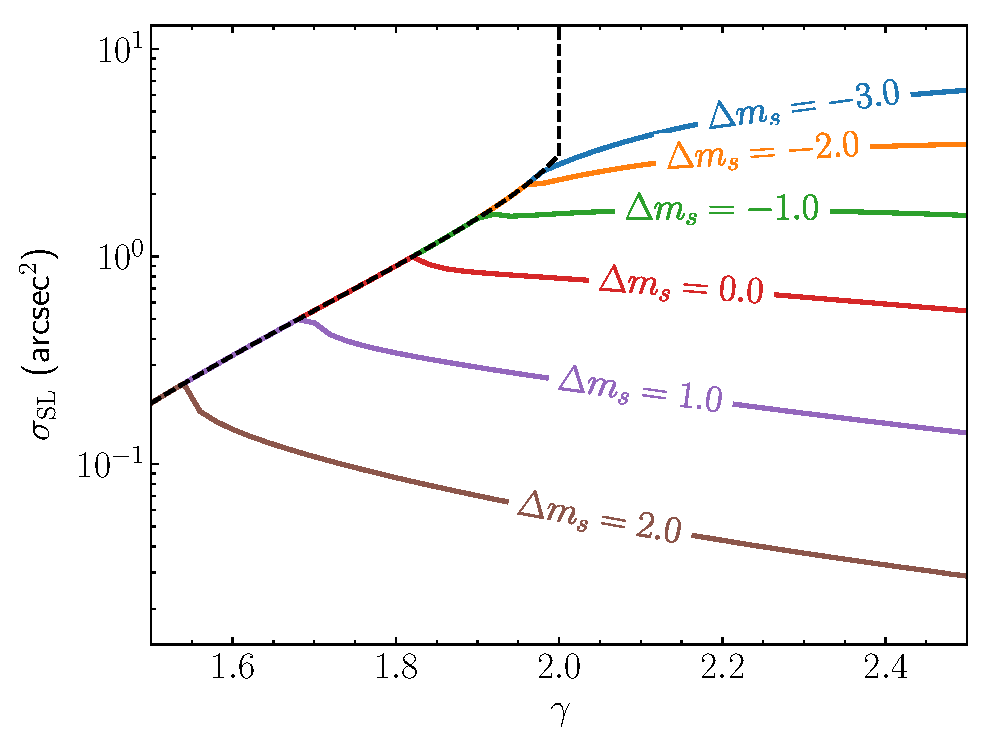
\includegraphics[width=\columnwidth]{axisymm_pl_crosssect.eps}
\caption{
Strong lensing cross-section of an axisymmetric power-law lens and a point source, as a function of the power-law slope $\gamma$.
The system is defined as a strong lens if at least two images are detected.
Different lines correspond to the difference $\Delta m$ between the source magnitude and the survey detection limit for a point source.
The dashed line marks the cross-section in the case in which at least two images are formed, regardless of their magnification.
}
\end{figure}

\subsection{Elliptical lenses, point sources}

\subsection{Elliptical lenses, extended sources}

%__________________________________________________________________

\section{Lens populations}\label{sect:lenspop}


%__________________________________________________________________

\section{Discussion and summary}\label{sect:discuss}

Discuss.

%\begin{acknowledgements}

%\end{acknowledgements}


\bibliographystyle{aa}
\bibliography{references}

\end{document}


